\section{Numbers}
\subsection{Natural numbers and integers}
In order to constract abstract algebra, we define the natural numbers, $\mathbb{N}$, and the integers, $\mathbb{Z}$, where
\begin{align*}
    \mathbb{N}&=\{0,1,2,3,4,5,\ldots\} \\
    \mathbb{Z}&=\{\ldots,-2,-1,0,1,2,\ldots\}
\end{align*}
Making $\mathbb{N}$ a subset of $\mathbb{Z}$, $\mathbb{N}\subset\mathbb{Z}$. In order to construct these as ordered sets, we define the greater than- or equal and  greater than operator, let $X,Y\in\mathbb{Z}$ then we define
\[
    X\leq Y\iff X-Y\in\mathbb{N}\hskip 16pt \text{and}\hskip 16pt X<Y\iff X\neq Y\vee X\leq Y
\]
Giving us the usual number ordering
\[
    \cdots<-3<-2<-1<0<1<2<3<\cdots
\]\vskip -10pt
\begin{defi}[First element]
    Let $s\in S$ where $S\subseteq\mathbb{Z}$, then $s$ is the unique first element in $S$ if $\forall x\in S,s\leq x$.
\end{defi}
\begin{exmp}
    Suppose that $S=\{1,2,3,4,\ldots\}$, then $\forall x\in S,1\leq x$, making $1$ the first element of the set.
\end{exmp}
It is immediately obvious that every nonempty subset of $\mathbb{N}$ must have a first element (due to it having a concrete lower bound), we call this property being well-ordered.
\pagebreak\subsection{Modular arithmetic}
Imagine that every multiple of 3 is marked on the axis of integers
\begin{figure}[!h]
    \centering
    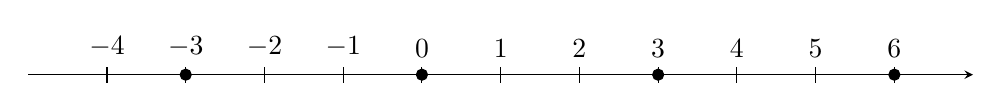
\begin{tikzpicture}
        \draw[-stealth] (-5,0) -- (7,0);
        \foreach \x in {-4,...,6}
            \draw (\x,-.1) -- (\x,.1) node[above]{$\x$};
        \foreach \y in {-3,0,...,6}
            \draw[fill=black] (\y,0) circle (2pt);
    \end{tikzpicture}
\end{figure}

then any integer can be expressed by the closest left multiple of 3 and the amount of you have to travel right to reach it.
We call the amount you walk to the right the remainder following division by 3.
\begin{exmp}
    Suppose we are observing multiples of 3, then
    \[
        5=3\times 1+2\hskip 32pt 7=3\times 2+1
    \]
    As such 5 has remainder 2 with respect to 3 and and 7 has remainder 1 with respect to 3.
\end{exmp}
\begin{theo}[Uniqueness of remainder]
    Let $d\in\mathbb{Z}$ where $d>0$, then $\forall x\in\mathbb{Z}$ there exists a unique remainder $r\in\mathbb{N}$ such that
    \[
        x=qd+r
    \]
    where $q\in\mathbb{Z}$ and $0\leq r<d$.
\end{theo}
\begin{prf}
    Assume that $x=q_{1}d+r_{1}$ and $n=q_{2}d+r_{2}$ where $q_{1},q_{2},r_{1},r_{2}\in\mathbb{Z}$ and $0\leq r_{1},r_{2}<d$ then
    \begin{align*}
        q_{1}d+r_{1}=q_{2}d+r_{2}&\implies q_{1}d-q_{2}d=r_{2}-r_{1} \\
                     &\implies d(q_{1}-q_{2})=r_{2}-r_{1}
    \end{align*}
    as we are assuming that $r_{1}\neq r_{2}$, we let $r_{2}$ be larger than $r_{1}$, which implies that $r_{2}-r_{1}=md$ where $m=q_{1}-q_{2}$, but this contradicts that $r_{2}-r_{1}\leq r_{2}<d$. To prove the existence of $r$, we let $M=\{x-qd~|~q\in\mathbb{Z}\}$, then $M\cap\mathbb{N}\neq\emptyset$, whereby $r$ must be the first element in $M\cap\mathbb{N}$, as such $\exists q,r=x-qd$, where $0\leq r<d$. If $r\geq d$ then $r>r-d\geq 0$ and $r-d=x-(q+1)d\in M\cap\mathbb{N}$, contradicting that $r$ is the first element in $M\cap\mathbb{N}$.
\end{prf}
\begin{defi}[Divisor]
    Suppose that $a=bc$ where $a,b,c\in\mathbb{Z}$, then we call $c$
    a divisor of $a$, which we write as $c\mid a$.
\end{defi}
\begin{defi}[Remainder]
    If $x,d\in\mathbb{Z}$ where $d>0$ we let $[x]_{d}$ be the unique remainder from Theorem 1.1.
\end{defi}
\pagebreak\subsection{Congruences}
\begin{defi}[Congruence]
    Let $a,b,c\in\mathbb{Z}$ then $a,b$ are called congruent modulo $c$ if $c\mid b-a$, denoted $a\equiv b\mod c$, which can be simply stated as them having the same remainder when divided by $c$.
\end{defi}
\begin{prop}[Congruence]
    Let $c\in\mathbb{Z}$ where $c>0$ then:
    \begin{itemize}
        \item[(i)] $a\equiv[a]_{c}\mod c$
        \item[(ii)] $a\equiv b\mod c\iff[a]_{c}=[b]_{c}$
    \end{itemize}
    for $a,b\in\mathbb{Z}$.
\end{prop}
\begin{prf}
    We know that $\exists q\in\mathbb{Z},a=qc+[a]_{c}$ by Theorem 1.1, whereby
    \begin{align*}
        a=qc+[a]_{c}&\implies a-[a]_{c}=qc \\
                    &\implies c\mid a-[a]_{c}=qc
    \end{align*}
    proving (i). We now define $b=q'c+[b]_{c}$ for some $q'\in\mathbb{Z}$, then
    \[
        a-b=(q-q')c+[a]_{c}-[b]_{c}
    \]
    whereby $c\mid a-b\iff c\mid[a]_{c}-[b]_{c}$ which as $0<[a]_{c},[b]_{c}<c\implies[a]_{c}=[b]_{c}$ proving (ii).
\end{prf}
\begin{exmp}
  The integers 29 and 14 can be written as $29=5\times 5+4$ and $14=5\times 2+4$, as they both have the same remainder
  \[
      [29]_{5}=[24]_{5}=4\iff 24\equiv 14\mod 5
  \]
\end{exmp}
\pagebreak\begin{prop}[Congruence of sum and product]
    Suppose that $x_{1}\equiv x_{2}\mod d$ and $y_{1}\equiv y_{2}\mod d$ then:
    \begin{itemize}
        \item[(i)] $x_{1}+y_{1}\equiv x_{2}+y_{2}\mod d$
        \item[(ii)] $x_{1}y_{1}\equiv x_{2}y_{2}\mod d$
    \end{itemize}
    for $x_{1},x_{2},y_{1},y_{2}\in\mathbb{Z}$.
\end{prop}
\begin{prf}
    Since $d$ divides $x_{1}-x_{2}$ and $y_{1}-y_{2}$, it must also divide the sum of the two
    \[
        d\mid x_{1}-x_{2}+y_{1}-y_{2}\implies d\mid x_{1}+y_{1}-(x_{2}+y_{2})
    \]
    proving (i). Similarly we recognize that
    \[
        x_{1}y_{1}-x_{2}y_{2}=x_{1}(y_{1}-y_{2})+y_{2}(x_{1}-x_{2})
    \]
    And as $x_{1},y_{2}$ are factors of terms we know to be divisible by $d$, so must their products be, and by (i) also their sum, proving (ii).
\end{prf}
\begin{exmp}
    We wish to determine the remainder of $12^{11}$ divided by 21. We split the exponent using binary expansion
    \[
        11=2^{3}+2^{1}+2^{0}=2^{3}+2+1
    \]
    From this it follows that $\left[12^{11}\right]=\left[\left[12^{2^{3}}\right]\left[12^{2}\right]\left[12\right]\right]$. As such we compute
    \begin{align*}
        \left[12^{1}\right]&=12 \\
        \left[12^{2}\right]&=18 \\
        \left[12^{2^{2}}\right]=\left[(12^{2})^{2}\right]=\left[12^{2}\left[12^{2}\right]\right]=\left[18\times 18\right]&=9 \ \\
        \left[12^{2^{3}}\right]=\left[\left(12^{2^{2}}\right)^{2}\right]=\left[\left[12^{2^{2}}\right]\left[12^{2^{2}}\right]\right]=\left[9\times 9\right]&=18
    \end{align*}
    Which lets us compute the remainder as
    \[
        \left[12^{11}\right]=\left[18\times 18\times 12\right]=3
    \]
\end{exmp}
\pagebreak\subsection{Greatest common divisor}
\begin{defi}[Divisor set]
    Let $D=\{d\in\mathbb{N}~|~d\mid n\}$ be the set of natural divisors of $n\in\mathbb{Z}$, we call $D$ the divisor set of $n$ and denote it $\text{div}(n)$.
\end{defi}
\begin{exmp}
    A few example are listed:
    \begin{align*}
        \text{div}(12)&=\{1,2,3,4,6,12\} \\
        \text{div}(28)&=\{1,2,4,14,28\} \\
        \text{div}(32)&=\{1,2,4,8,16,32\}
    \end{align*}\vskip -10pt
\end{exmp}
Here an interesting pattern emerges when we determine the intersection of divisor sets:
\begin{align*}
    \text{div}(12)\cap\text{div}(28)&=\{1,2\}=\text{div}(2) \\
    \text{div}(28)\cap\text{div}(32)&=\{1,2,4\}=\text{div}(4)
\end{align*}
Indicating that the intersection of divisor sets for some $m,n\in\mathbb{Z}$ form a divisor set for a third number $d\in\mathbb{N}$.
\begin{lemm}[Euclid]
    Let $m,n\in\mathbb{Z}$, then there exists a unique natural number $d\in\mathbb{N}$ such that
    \[
        \text{div}(m)\cap\text{div}(n)=\text{div}(d)
    \]
\end{lemm}
\begin{prf}
    Uniqueness follows from the fact that no two distinct natural numbers have the same divisior sets as it always contains itself. To prove existence of $d$ we assume that $m,n\in\mathbb{N}$, since $\text{div}(x)=\text{div}(-x)$ for $x\in\mathbb{Z}$. We use induction on $\min(m,n)$ where
    \[
        \min(m,n)=m\implies m\leq n\text{ and }\min(m,n)=n\implies m>n
    .\]
    If $\text{min}(m,n)=0$, we can assume that $n=0$ whereby $\text{div}(m)\cap\text{div}(n)=\text{div}(m)$ as all numbers divide zero whereby $\text{div}(m)\subset\text{div}(0)$. We now assume that $\text{div}(m)\cap\text{div}(n)=\text{div}(d)$ holds for every $m,n\in\mathbb{N}$ where $\min(m,n)<N$ with $N>0$.

    Using induction, we suppose that $m,n\in\mathbb{N}$ where $\min(m,n)=N$ with $m\geq n=N$. Then we have that $\exists q\in\mathbb{Z},m=qn+r$ where $0\leq r<n$ by Theorem 1.2.1, then 
    \[
        \text{div}(m)\cap\text{div}(n)=\text{div}(m-qn)\cap\text{div}(n)=\text{div}(r)\cap\text{div}(n)
    \]
    as a number divides $m,n$ if and only if it also divides $m-qn$. By induction we know that $\text{div}(r)\cap\text{div}(n)=\text{div}(d)$ for some $d\in\mathbb{N}$ since $\min(r,n)=r<n=N$.
\end{prf}
\begin{defi}[Greatest common divisor]
    The unique number $d\in\mathbb{N}$ discussed above is called the greatest common divisor of $m,n$ denoted $d=\text{gcd}(m,n)$.
\end{defi}
\pagebreak\subsection{Euclidean algorithm}
% Lemma 1.4.1 indicates that an algorithm to compute the greatest common divisor exists, which is of course the case.
\begin{prop}[Euclid's algorithm]
    Let $m,n\in\mathbb{N}$, then:
    \begin{itemize}
        \item[(i)] $\text{gcd}(m,0)=m$ if $m\in\mathbb{N}$.
        \item[(ii)] $\text{gcd}(m,n)=\text{gcd}(m-qn,n)$ for every $q\in\mathbb{Z}$.
    \end{itemize}
\end{prop}
\begin{prf}
    As $\text{div}(0)=\mathbb{Z}\implies\text{gcd}(m,0)=\text{div}(m)\cap\text{div}(\mathbb{Z})=\text{div}(m)$, proving (i). We arrive at (ii) from the fact that
    \[
        \text{div}(d)=\text{div}(m)\cap\text{div}(n)=\text{div}(m-qn)\cap\text{div}(n)
    \]
    being an alternative way to express that $d\mid m,n\iff d\mid m-qn,n$, such that $\text{gcd}(m,n)=\text{gcd}(m-qn,n)$.
\end{prf}
\begin{exmp}
    Let $m=24$ and $n=14$, then
    \[
        \text{gcd}(24,14)=\text{gcd}(14,10)=\text{gcd}(10,4)=\text{gcd}(4,2)=\text{gcd}(2,0)=2
    \]\vskip -10pt
\end{exmp}
For a more general case with $m\leq n\leq 0$, we let $r_{-1}=m$ and $r_{0}=n$, if $r_{0}=0$ then $\text{gcd}(r_{-1},r_{0})=r_{-1}$, if this is not the case however then we define $r_{1}=[r_{-1}]_{r_{0}}\implies \exists q_{1},r_{1}=r_{-1}-q_{1}r_{0}$, wherby we let $\text{gcd}(r_{-1},r_{0})=\text{gcd}(r_{0},r_{1})$, repeating until $r_{N}=0$ whereby we have that $\text{gcd}(m,n)=r_{N-1}$.

Since $m,n$ share a common factor, it must be possible to construct a linear combination of $m,n$ resulting in said factor.
\begin{exmp}
    We wish to determine $\lambda,\mu\in\mathbb{Z}$ such that $\lambda\times 24+\mu\times 14=2$, we do this by determining $\lambda,\mu$ for the remainder in each step of the algorithm
    \begin{align*}
        24&=1\times 24+0\times 14 \\
        14&=0\times 24+1\times 14 \\
        10&=24-14=1\times 24-1\times 14 \\
        4&=14-10=-1\times 24+2\times 14 \\
        2&=10-2\times 4=24-14=2\times 24-3\times 14
    \end{align*}
    Whereby $2\times 24-3\times 14=\text{gcd}(n,m)$.
\end{exmp}
\begin{defi}[Extended Euclidean algorithm]
    The Euclidean algorithm with the addition demonstrated above for computing $\lambda,\mu$ is called the extended Euclidean algorithm.
\end{defi}
\begin{lemm}[Linear combination exists]
    Let $m,n\in\mathbb{Z}$, then there exist $\lambda,\mu\in\mathbb{Z}$ such that
    \[
        \lambda m+\mu n=\text{gcd}(m,n)
    .\]\vskip -10pt
\end{lemm}
\begin{prf}
    Let $m,n\in\mathbb{N}$ and $d=\text{gcd}(m,n)$, then the extended Euclidean algorithm will give $\lambda,\mu\in\mathbb{Z}$ such that $\lambda m+\mu n=d$, we now show that
    \[
        (-\lambda)(-m)+\mu n=\lambda m+(-\mu)(-n)=(-\lambda)(-m)+(-\mu)(-n)=d
    \]
    Showing that $\lambda,\mu$ exist for all $m,n$.
\end{prf}\vskip -10pt
\begin{defi}[Coprime integers]
    Two integers $a,b\in\mathbb{Z}$ are called relatively prime (or coprime) if
    \[
        \text{gcd}(a,b)=1
    .\]\vskip -10pt
\end{defi}
\begin{coro}[Divisor of product of relative prime]
    Suppose that $a\mid bc$ where $a,b,c\in\mathbb{Z}$ where $\text{gcd}(a,b)=1$, then $a\mid c$.
\end{coro}
\begin{prf}
    By Lemma 1.5.1 there exists a linear combination $\lambda a+\mu b=1$, multiplying by $c$ then gives $\lambda ac+\mu bc=c\implies a\mid c$ as $a$ obviously divides the first term and $bc$ by the proposition.
\end{prf}\vskip -10pt
\begin{coro}[Properties of relative primes]
    Let $a,b,c\in\mathbb{Z}$ then:
    \begin{itemize}
        \item[(i)] If $\text{gcd}(a,b)=1$, $a\mid c$ and $b\mid c$ then $ab\mid c$.
        \item[(ii)] If $\text{gcd}(a,b)=1$ and $\text{gcd}(a,c)=1$ then $\text{gcd}(a,bc)=1$.
    \end{itemize}
\end{coro}
\begin{prf}
    By Lemma 1.5.1 there exists a linear combination $\lambda a+\mu b=1$, since $a,b\mid c$ we can write $c$ as $c=ax=by$ for some $x,y\in\mathbb{Z}$, as such we multiply the linear combination by $c$, giving
    \[
        c=\lambda ac+\mu bc=\lambda aby+\mu bax=ab(\lambda y+\mu x)
    \]
    proving (i). To prove (ii) we again use Lemma 1.5.7, whereby we get two identities $\lambda_{1}a+\mu_{1}b=1$ and $\lambda_{2}a+\mu_{2}c=1$ for some $\lambda_{1},\mu_{1},\lambda_{2},\mu_{2}\in\mathbb{Z}$,  multiplying the two together we have that
    \[
        1=(\lambda_{1}a+\mu_{1}b)(\lambda_{2}a+\mu_{2}c)=(\lambda_{1}\lambda_{2}a+\lambda_{1}\mu_{2}c+\mu_{1}b\lambda_{2})a+(\mu_{1}\mu_{2})bc
    \]
    Showing that $\text{gcd}(a,bc)=1$ whereby they are relative primes.
\end{prf}
\pagebreak\subsection{Chinese remainder theorem}
\begin{exmp}
 Consider a number $x<30$, let $a,b,c$ be rows numbered upwards from zero in the following three tables where the number is located
\\\\\begin{centering}\begin{tabular}{|ccccccccccccccc|}
    \hline
    0 & 2 & 4 & 6 & 8 & 10 & 12 & 14 & 16 & 18 & 20 & 22 & 24 & 26 & 28 \\
    \hline
    1 & 3 & 5 & 7 & 9 & 11 & 13 & 15 & 17 & 19 & 21 & 23 & 25 & 27 & 29 \\
    \hline
\end{tabular}

\begin{tabular}{|cccccccccc|}
    \hline
    0 & 3 & 6 & 9 & 12 & 15 & 18 & 21 & 24 & 27 \\
    \hline
    1 & 4 & 7 & 10 & 13 & 16 & 19 & 22 & 25 & 28 \\
    \hline
    2 & 5 & 8 & 11 & 14 & 17 & 20 & 23 & 26 & 29 \\
    \hline
\end{tabular}

\begin{tabular}{|cccccc|}
    \hline
    0 & 5 & 10 & 15 & 20 & 25 \\ 
    \hline
    1 & 6 & 11 & 16 & 21 & 26 \\
    \hline
    2 & 7 & 12 & 17 & 22 & 27 \\
    \hline
    3 & 8 & 13 & 18 & 23 & 28 \\
    \hline
    4 & 9 & 14 & 19 & 24 & 29 \\
    \hline
\end{tabular}\\\end{centering}\vskip 10pt
Take for example $x=27$, then we find $a=1,b=0,c=2$, in fact, these numbers are all you need to know in order to determine $x$, this is called the 30-riddle.
\end{exmp}
\begin{defi}[Remainder map]
    Define
    \[
        \mathbb{Z}/N=\{X\in\mathbb{N}~|~0\leq X<N\}
    \]
    For $N\in\mathbb{N}$. If $N=n_{1}\times n_{2}\times\ldots\times n_{t}\neq 0$ then we let
    \[
        r:\mathbb{Z}/N\rightarrow\mathbb{Z}/n_{1}\times\cdots\times\mathbb{Z}/n_{t}
    \]
    By the map given by $r(X)=([X]_{n_{1}},\ldots,[X]_{n_{t}})$. We call this the remainder map.
\end{defi}
\begin{exmp}
  Suppose that $N=2\times 3\times 5=30$ and $x=27$, then we have that
  \[
      r(27)=\left([27]_{2},[27]_{3},[27]_{5}\right)=(1,0,2)
  \]
  We recognize this tuple as the values $a,b,c$ for $x=27$ in the 30-riddle.
\end{exmp}
\begin{lemm}[Bijective remainder map]
    Suppose that $N=n_{1}\times n_{2}\times\cdots\times n_{t}$ where $n_{1},n_{2}\ldots,n_{t}\in\mathbb{N}\setminus\{0\}$ and $\text{gcd}(n_{i},n_{j})=1$ if $i\neq j$ then
    \[
        r:\mathbb{Z}/N\rightarrow\mathbb{Z}/n_{1}\times n_{2}\times\cdots\times n_{t}
    \]
    is bijective.
\end{lemm}
\begin{prf}
    If $r(X)=r(Y)$ then $[X]_{n_{i}}=[Y]_{n_{i}}$ for all $i\in\{1,2,\ldots,t\}$, implying that $X\equiv Y\mod n_{i}$ whereby $n_{i}\mid X-Y$. From Corollary 1.5.2 we know that if $\text{gcd}(a,b)=1$ and $\text{gcd}(a,c)=1$ then $\text{gcd}(a,bc)=1$, meaning that if a number is divisible by several coprimes, it is also divisible by their products, and as such $N\mid X-Y$. Similarly we recognize that $0\leq X,Y<N$, whereby it is only possible for $N$ to divide $X-Y$ if their sum is equal 0, and as such $X=Y$, implying that each mapping is unique and $r$ is therewfore injective, this implies that $r$ is also surjective as the codomain and domain have the same number of elements, making $r$ injective.
\end{prf}
\begin{theo}[Chinese remainder theorem]
    Suppose that $N=n_{1}\times n_{2}\times\cdots\times n_{t}$ where $n_{1},n_{2},\ldots,n_{t}\in\mathbb{Z}\setminus\{0\}$ and $\text{gcd}(n_{i},n_{j})=1$ for $i\neq j$. Consider the system of congruences
    \begin{align*}
        X&\equiv a_{1}\mod n_{1} \\
      X&\equiv a_{2}\mod n_{2} \\
       &\vdotswithin{\equiv} \\
      X&\equiv a_{t}\mod n_{t}
    \end{align*}
    for $a_{1},a_{2},\ldots,a_{t}\in\mathbb{Z}$. Then:
    \begin{itemize}
        \item[(i)] The system has a solution $X\in\mathbb{Z}$.
        \item[(ii)] If $X,Y\in\mathbb{Z}$ are solutions of the system then $X\equiv Y\mod N$. If $X$ is a solution and $Y\equiv X\mod N$ then $Y$ is a solution.
    \end{itemize}
\end{theo}
\begin{prf}
    If $X,Y$ are solutions then by Lemma 1.6.1 $N\mid X-Y$ and $X\equiv Y\mod N$, the same applies in reverse where $Y\equiv X\mod N$ and $N\mid Y-X$, proving (ii) by showing theyre both solutions. As we know $n_{i}$ and $N/n_{j}$ must be relatively prime ($N/n_{j}$ contains the product of the other coprime terms without $n_{j}$) there must exist integers $\lambda_{j},\mu_{j}$ such that
    \begin{align*}
        \lambda_{1} n_{1}+\mu_{1}N/n_{1}&=1 \\
        \lambda_{2}n_{2}+\mu_{2}N/n_{2}&=1 \\
                                       &\vdotswithin{\equiv} \\
        \lambda_{t}n_{t}+\mu_{t}N/n_{t}&=1
    \end{align*}
    We let $A_{j}=\mu_{j}N/n_{j}$ for $j=\{1,2,\ldots,t\}$ noticing that $A_{j}\mod n_{j}=1$ and $A_{j}\mod n_{i}=0$ for $i\neq j$, we build a solution from these as
    \[
        X=a_{1}A_{1}+a_{2}A_{2}+\cdots+a_{t}A_{t}
    \]
    Where we can ignore the first term it is equal 1 when the other term is equal 0 and vice versa, whereby the equation.
\end{prf}
\begin{exmp}
    Applying the above on the 30-riddle we have that $n_{1}=2,n_{2}=3,n_{3}=5$, we find $\lambda_{i},mu_{i}\in\mathbb{Z}$ that satisfy
    \begin{align*}
        \lambda_{1}n_{1}+\mu_{1}N/n_{1}&=2\lambda_{1}+(2\times 3\times 5)/2\mu_{1}=2\lambda_{1}+15\mu_{1}=1 \\
        \lambda_{2}n_{2}+\mu_{2}N/n_{2}&=3\lambda_{2}+(2\times 3\times 5)/3\mu_{2}=3\lambda_{2}+10\mu_{2}=1 \\
        \lambda_{3}n_{3}+\mu_{3}N/n_{3}&=5\lambda_{3}+(2\times 3\times 5)/5\mu_{3}=5\lambda_{3}+6\mu_{3}=1
    \end{align*}
    Which has solution $\lambda_{1}=-7,\mu_{1}=1,\lambda_{2}=-3,\mu_{2}=1,\lambda_{3}=-1,\lambda_{3}=1$, giving us $A_{1}=15,A_{2}=10,A_{3}=6$ whereby
    \[
        X=15a_{1}+10a_{2}+6a_{3}
    \]
    Is a solution to the system of congruences
    \begin{align*}
        X&\equiv a_{1}\mod 2
        X&\equiv a_{2}\mod 3
        X&\equiv a_{3}\mod 5
    \end{align*}
    And as such we can determine our original number using $a_{1},a_{2},a_{3}$, for $a_{1}=1,a_{2}=0,a_{3}=2$ we find that $X=15+0+12=27$, and determine the remainder following division by 30 $[X]_{30}=[27]_{30}=27$, which is also the number we used in the first example.
\end{exmp}
